\documentclass[a4paper,twoside,master.tex]{subfiles}
\begin{document}
\lecture{3}{Wednesday, January 15, 2020}{Probability Densities}

A useful consequence of Stirling's approximation is
\begin{equation}
    \ln{\binom{n}{k}} = -n\left[ \varphi \ln{\varphi} + (1 - \varphi) \ln{1 - \varphi} \right] \quad \varphi = \frac{k}{n}
\end{equation}

\section{Continuous Random Variables}
\label{sec:continuous_random_variables}

Instead of asking for the probability to get a particular point, we instead ask about the probability of covering regions in event space.

\begin{ex}
    Let $ x \in \R $ be uniformly picked between $ 0 $ and $ 10 $. What is the probability that $ x \in \left[ 7,9 \right] $?
    \begin{equation}
        \Pr(7 \leq x \leq 9) = \frac{2}{10}
    \end{equation}
    \begin{equation}
        \Pr(x = 8) \text{ is meaningless in general}
    \end{equation}

    We can also define probability densities:
    \begin{equation}
        \Pr(x) = \begin{cases} \frac{1}{10} & x \in \left[ 0, 10 \right] \\ 0 & x \notin \left[ 0, 10 \right] \end{cases}
    \end{equation}

    In this case,
    \begin{equation}
        \Pr(7 \leq x \leq 9) = \int_7^9 \dd{x} \Pr(x) = 0.2
    \end{equation}
    This does not mean $ \Pr(8) = \frac{1}{10} $, since we need to integrate over this density.
\end{ex}

In general, integrals of probability densities are probabilities. For $ x \in \Omega $, the probability density is always non-negative ($ \Pr(x) \geq 0 $). Normalization gives us $ \int_{\Omega} \dd{x} \Pr(x) = 1 $.

\begin{itemize}
    \item We also require $ \dd{x} \Pr(x) $ to be dimensionless, so $ \left[ \Pr(x) \right] = \frac{1}{\left[ \dd{x} \right]} $. Note that the notation for probability density is identical to the notation for a probability, so we must be cautious when deciding which is meant.
    \item Since probability densities generally have units, their numerical values need not be smaller than $ 1 $.
    \item Probability densities can also diverge\textemdash their values can become infinite, as long as the integral is well-defined.
        \begin{ex}
            \begin{equation}
                \Pr(x) = \begin{cases} \frac{1}{2 \sqrt{x}} & 0 < x \leq 1 \\ 0 \qotherwise \end{cases}
            \end{equation}
            Notice that
            \begin{equation}
                \int_0^1 \dd{x} \Pr(x) = \eval{\sqrt{x}}_0^1 = 1
            \end{equation}
            so there is no problem with the divergence at $ 0 $.
        \end{ex}
    \item All of our knowledge of discrete random variables carries over with $ \sum \to \int $ and $ \delta_{ij} \to \delta(x-y) $.
        \begin{ex}
            If we have a random variable $ x \in \mathbb{D} $ with a probability density $ \Pr_{X}(x) $ and a function $ F(x) $, what is the probability density $ \Pr_{F}(f) $? We can extend transformation theorem to show that
            \begin{equation}\label{eq:transformation_prob_density}
                \Pr_{F}(f) = \int_{\mathbb{D}} \dd{x} \delta(f-F(x)) \Pr_{X}(x)\tag{Transformation Theorem for Probability Densities}
            \end{equation}
            Note that this integral does not simplify in general because the $\delta$-function contains a function of $ x $ instead of just $ x $. One option to simplify this is to make a variable substitution for $ F(x) $, but this only works in regions where $ F(x) $ is invertible.
        \end{ex}
\end{itemize}

\section{Ideal Gasses}
\label{sec:ideal_gasses}

By ``ideal'' we mean that gas atoms or molecules do not interact:
\begin{equation}
    H = \sum_{i=1}^{N} \frac{p_i^2}{2m}
\end{equation}

It is reasonable to assume in this case that the positions are independent of the momenta (a very classical assumption).
\begin{equation}
    \Pr(\{q_1, q_2,\cdots,q_N,p_1, p_2,\cdots,p_N\}) = \Pr_{q}(\{q_1, \cdots, q_N\}) \Pr_{p}(\{p_1, \cdots, p_N\})
\end{equation}
In shorthand, we will write $ \Pr(q,p) = \Pr_{q}(q) \Pr_{p}(p) $. We will treat these terms separately, and for now, we will concern ourselves with the position.

For an ideal gas, we may further assume that all positions are independent of one another.
\begin{equation}
    \Pr_{q}(q) = \prod_{i=1}^{N} \Pr_{q_i}(q_i) = \prod_{i=1}^{N} \Pr_{q_1}(q_i)
\end{equation}
since we also assume the particles are identically distributed. Notice that the second term requires an Avogadro's number of probability densities, while the final term  only requires one.

Let's now imagine an isolated box divided into two compartments with a hole in the division. We have gas particles in both sides, and because of the hole, they can move from the left side to the right side and back. The left side has $ N_A $ particles, volume $ V_A $, and energy $ E_A $, while the right hand side has $ N_B $, $ V_B $, and $ E_B $, where
\begin{align}
    N_A + N_B &= N \\
    V_A + V_B &= V \\
    E_A + E_B &= E
\end{align}

\begin{figure}[h]
    \centering
    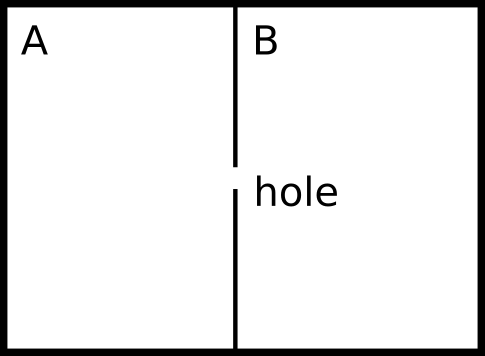
\includegraphics[width=\textwidth/2]{figures/lec_03_box_with_hole.png}
    \caption{Box with hole}
    \label{fig:box_with_hole}
\end{figure}

For any given particle, what is the probability of a particular particle being in compartment $ A $?
\begin{equation}
    \Pr = \frac{V_A}{V}
\end{equation}

Why is this true? Physicists call this the equal a priori principle. We are assuming these particles are evenly distributed in this box. If we make this assumption, we can later derive predictions, and as it turns out, an incredible amount of nontrivial things can be predicted and experimentally verified.



\end{document}
